% !TeX program = pdfLaTeX
\documentclass[12pt]{article}
\usepackage{amsmath}
\usepackage{graphicx,psfrag,epsf}
\usepackage{enumerate}
\usepackage{natbib}
\usepackage{textcomp}
\usepackage[hyphens]{url} % not crucial - just used below for the URL
\usepackage{hyperref}

%\pdfminorversion=4
% NOTE: To produce blinded version, replace "0" with "1" below.
\newcommand{\blind}{0}

% DON'T change margins - should be 1 inch all around.
\addtolength{\oddsidemargin}{-.5in}%
\addtolength{\evensidemargin}{-.5in}%
\addtolength{\textwidth}{1in}%
\addtolength{\textheight}{1.3in}%
\addtolength{\topmargin}{-.8in}%

%% load any required packages here



% tightlist command for lists without linebreak
\providecommand{\tightlist}{%
  \setlength{\itemsep}{0pt}\setlength{\parskip}{0pt}}

% From pandoc table feature
\usepackage{longtable,booktabs,array}
\usepackage{calc} % for calculating minipage widths
% Correct order of tables after \paragraph or \subparagraph
\usepackage{etoolbox}
\makeatletter
\patchcmd\longtable{\par}{\if@noskipsec\mbox{}\fi\par}{}{}
\makeatother
% Allow footnotes in longtable head/foot
\IfFileExists{footnotehyper.sty}{\usepackage{footnotehyper}}{\usepackage{footnote}}
\makesavenoteenv{longtable}



\begin{document}


\def\spacingset#1{\renewcommand{\baselinestretch}%
{#1}\small\normalsize} \spacingset{1}


%%%%%%%%%%%%%%%%%%%%%%%%%%%%%%%%%%%%%%%%%%%%%%%%%%%%%%%%%%%%%%%%%%%%%%%%%%%%%%

\if0\blind
{
  \title{\bf Modeling K-12 school shootings as a clustered point process and an areal process, from 1990-2019}

  \author{
        J Steven Raquel \\
    Department of Statistics, University of California, Irvine\\
      }
  \maketitle
} \fi

\if1\blind
{
  \bigskip
  \bigskip
  \bigskip
  \begin{center}
    {\LARGE\bf Modeling K-12 school shootings as a clustered point process and an areal process, from 1990-2019}
  \end{center}
  \medskip
} \fi

\bigskip
\begin{abstract}
The prevalence of gun violence in schools in the United States has been referred to both as an epidemic and a public health crisis, and one that has steadily increased over the past several decades (see Figure \ref{fig:ts-plot-1990-2019}). The debate on how to curb these tragedies is a solidly partisan issue, with calls for more and stronger gun control laws, as well as more mental health care, sometimes as an alternative to gun control. Concealed carry laws are argued both in favor of, and against and are labeled as both an enabler and a potential deterrent to mass shootings. Apart from the trauma that such an event can bring to a community, there is also resonant fear that such incidents inspire copycat events on a local and a larger scale. This spatial analysis attempts to model the incidence of these shootings as a Poisson point process, in order to ascertain whether the locations and events occur with complete spatial randomness. We also model the data in an areal form on a per-state basis so as to compare it against the level of gun control and mental health care, also on a state level.
\end{abstract}

\noindent%
{\it Keywords:} Spatial statistics, Poisson point process, Areal data, mental health, gun violence, gun control
\vfill

\newpage
\spacingset{1.45} % DON'T change the spacing!

\hypertarget{data}{%
\section{Data}\label{data}}

The school shooting data was sourced directly from the ``K-12 School Shooting Database'' made available by the Center for Homeland Defense and Security (CHDS). The information that comprises the dataset was determined by a specific process which entailed asking what exactly comprises a school shooting. Most shootings that were premeditated and resulted in mass casualties, such as those that occurred at Columbine in 1999, Sandy Hook in 2012, and Stoneman Douglas in 2018, are considered ``indiscriminate shootings''. Although the original database contains shootings ruled accidental (from misuse of a firearm) as well as incidences of gang-related gun violence on school grounds, among other incidents, we did not opt to consider this data as relevant to this study in particular.

\begin{figure}
\centering
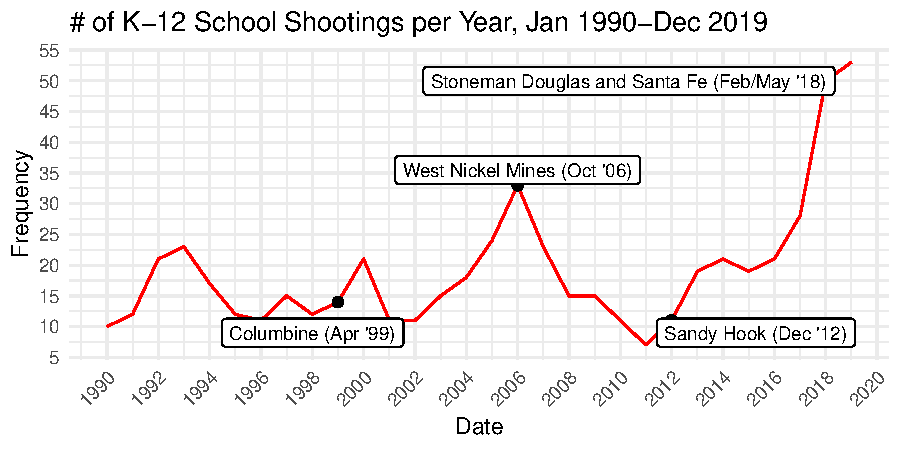
\includegraphics{JStevenRaquel_STATS295_Final_files/figure-latex/ts-plot-1990-2019-1.pdf}
\caption{\label{fig:ts-plot-1990-2019}Time series plot of number of K-12 school shootings per year, from Jan 1990 to Dec 2019.}
\end{figure}

It was a deliberate decision on our part to filter out these incidents as others like it so as to hone in one the more specific and cultural recognized definition of a school shooting, which is an attack that takes place on school grounds, in order to target students, faculty, or passersby with the intent to cause terror and/or inflict harm on specific individuals. Targeted events related to domestic situations (e.g.~anger over a break-up), or the escalation of disputes (e.g.~fistfights in which one person pulls out a firearm) were also ruled school shootings.

The database originally goes as far back as 1970 all the way to present day (March 2022 at the time of this writing), but it was of particular interest to look at the data after 1990 since this consolidates the modern era in which access to firearms and the incidence of gun violence in schools is more normalized. It was also decided to leave out data past 2019 as the COVID-19 pandemic which hit the US in 2020 is a huge confounding variable as it caused many schools to institute remote learning which decreased the incidence of shootings on school campuses.

The data originally only contained the name of the school, as well as the city and state where the events took place, but we were able to use the Google Maps API to source the specific latitude/longitude coordinates of these events.

In addition to this school shooting data, we also have gun control data consisting of several columns of binary categorical data as to whether or not a certain law (e.g.~a ban on concealed carry, background checks) is instituted in a given state for the years between 1991 and 2020 from StateFirearmLaws.org, as well as mental healthcare data from 2019 courtesy of Mental Health America (MHA), which consists of a ranking of all 50 states and the District of Columbia on their ratio of need for and accessibility to mental healthcare. More information on these resources can be found on their respective websites (see References section).

\hypertarget{methods}{%
\section{Methods}\label{methods}}

\hypertarget{exploratory-data-analysis}{%
\subsection{Exploratory Data Analysis}\label{exploratory-data-analysis}}

As a preliminary analysis, we chose to plot this data on both a point and at an areal level, for a number of reasons. For one, modeling the data as a point pattern allows us to test the null hypothesis for complete spatial randomness against the alternative hypothesis of clustering. It allows us to hone in on exactly where within a given state might be considered a ``hotspot'' for a shooting. Conversely, the areal data allows us to compare the number of incidents in a given state and look at it with respect to the level of gun control and mental healthcare available there as well.

\begin{figure}
\centering
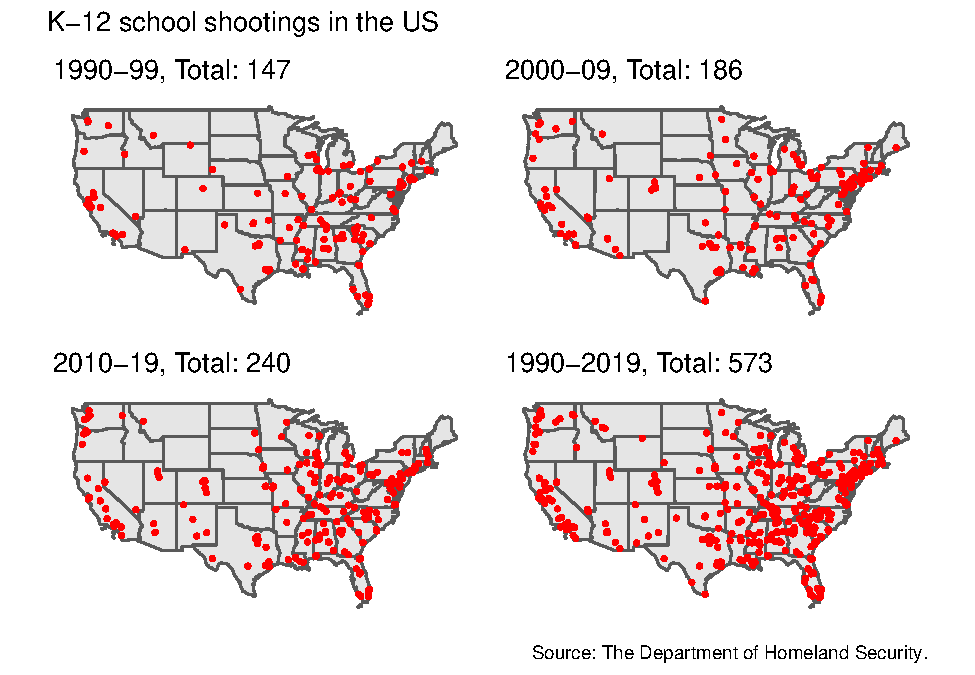
\includegraphics{JStevenRaquel_STATS295_Final_files/figure-latex/plots-all-four-1.pdf}
\caption{\label{fig:plots-all-four}Point pattern data for the three separate decades as well as all 30 years.}
\end{figure}

As we can see from Figure \ref{fig:plots-all-four}, the total number of shootings per decade has not only steadily increased over the past 30 years, but the events also occur in and around the same places, which gives credence to our hypothesis that the events exhibit a clustered point pattern. We notice in fact, that there are areas that seem relatively untouched by school shootings in the western United States, whereas shootings all across the South, Midwest and the East Coast recur at a frightening rate. While the West Coast is somewhat blighted by school shootings, particularly in the San Francisco and Los Angeles metropolitan areas, along with major cities in the Pacific Northwest), it is not nearly at the rate experience by the other side of the US.

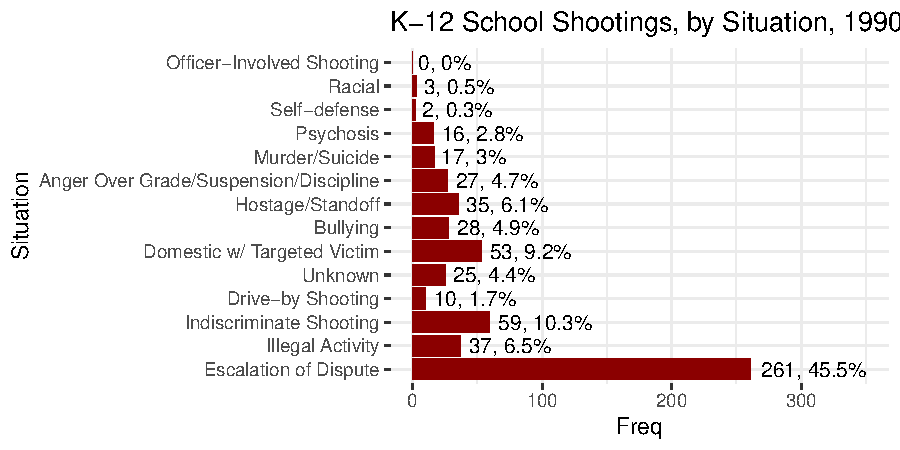
\includegraphics{JStevenRaquel_STATS295_Final_files/figure-latex/plot-situation-1.pdf}

\begin{figure}
\centering
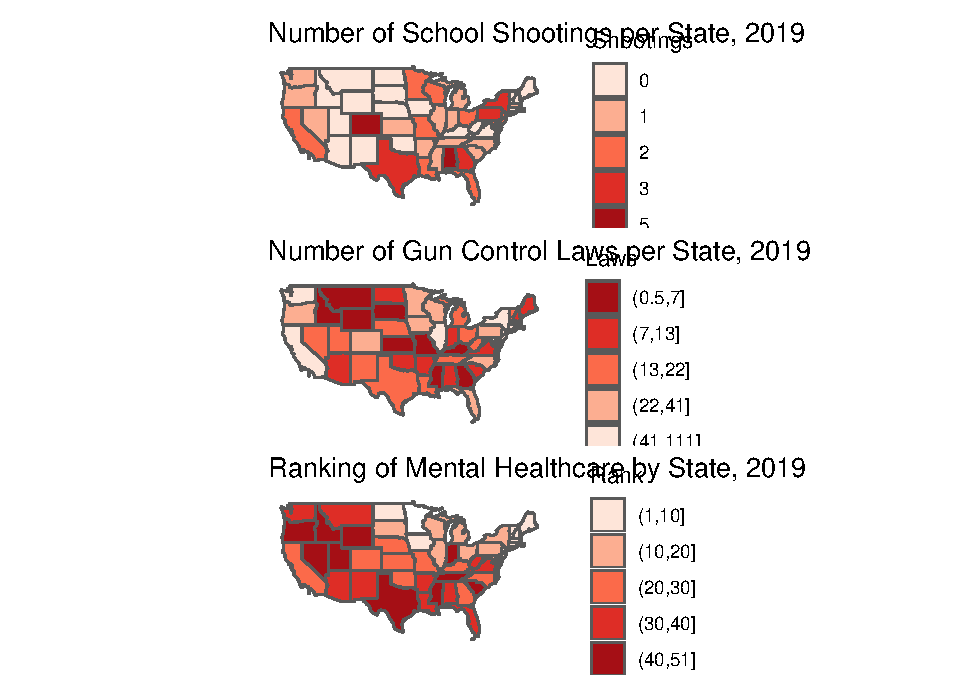
\includegraphics{JStevenRaquel_STATS295_Final_files/figure-latex/plot-areals-2019-1.pdf}
\caption{\label{fig:plot-areals-2019}A comparison of the incidence of school shootings against gun control and mental health care, in 2019.Darker shades of red imply more shootings, less gun control laws, and less access to mental healthcare.}
\end{figure}

\hypertarget{areal-data-visualization}{%
\subsection{Areal Data Visualization}\label{areal-data-visualization}}

Looking at Figure \ref{fig:plot-areals-2019}, we see that despite the conspicuous lack of gun control or adequate mental healthcare in the northwestern United States, e.g.~Idaho, Wyoming, Montana, there were few to no school shootings events in 2019, which is consistent with what we saw in the point pattern visualization as well. This may lend credence to a hypothesis that in fact, a lack of gun control laws and/or mental healthcare may not coincide with a greater incidence of shootings at all. 2019 was selected as the year to analyze in this fashion because it was the year with the highest number of shootings between 1990 and 2019.

Conversely, we do note that many states in the southern region of the US, e.g.~Texas, Mississippi, Alabama, do experience greater levels of gun violence in tandem with their lack of gun control or mental healthcare relative to other parts of the country.

A subset of the northeastern US shows an interesting pattern in that there were states with absolutely no school shootings (Maine, Vermont, New Hampshire) in 2019 despite a lack of strong gun control, but this was in fact in tandem with a relatively high ranking of access to mental healthcare.

The remainder of this literature will focus on the clustering Poisson point process model for the data, but analysis on an areal level will be left open-ended as potential future work to explore.

\hypertarget{point-pattern-analysis}{%
\subsection{Point Pattern Analysis}\label{point-pattern-analysis}}

With respect to the coordinate-level data, as with any spatial point pattern analysis, we are concerned with the following three questions, 1) whether the points are located at random, 2) whether they are clustered, and 3) whether they are placed regularly. The hypothesis of \emph{complete spatial randomness} (CSR) asserts the following:

\begin{itemize}
\tightlist
\item
  The number of events in any region \(S\) with area \(|S|\) follows a Poisson distribution with mean \(\lambda |S|\), where \(\lambda\) is the intensity, i.e.~\(\lambda\) does not change over \(S\)
\item
  Given \(n\) events in \(S\), the points \(s_i\) are independently located according to the uniform distribution on \(S\), i.e.~there is no interaction amongst events.
\end{itemize}

The intensity function \(\lambda(s)\), also known as the first-order property of the spatial point process, is defined as

\[\lambda(s) = \lim_{|\Delta s| \to 0} \frac{E[N(\Delta s)]}{| \Delta s|}\]

Firstly we want to ascertain whether the incidences of school shootings are indeed a Poisson process, and if so, determine whether or not the process is homogeneous (where the intensity function \(\lambda(s)\) assumes a constant \(\lambda\)) or inhomogeneous. The intensity function is the expected number of events per unit area, so a constant \(\lambda\) would mean that the events occur at a consistent rate across the whole spatial area. This could be in a patterned fashion, or completely random.

\hypertarget{quadrats}{%
\subsection{Quadrats}\label{quadrats}}

While we could estimate the intensity function across the entire area, what we are interested in this particular analysis is to how the intensity varies across different regions contained therein. We do this by splitting up the area into what are referred to as \emph{quadrats}.

\begin{figure}
\centering
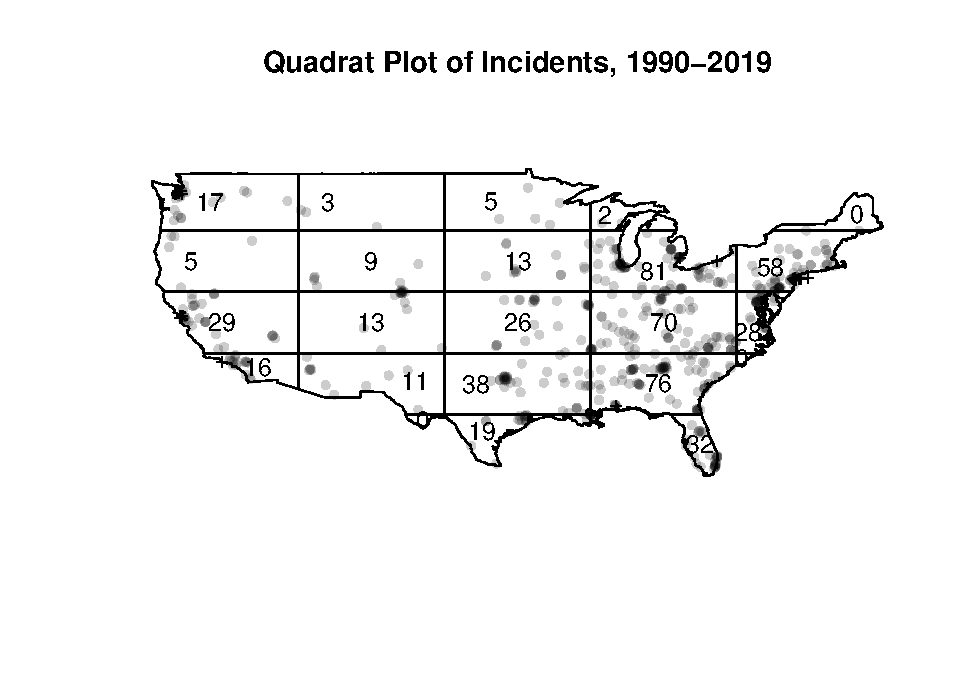
\includegraphics{JStevenRaquel_STATS295_Final_files/figure-latex/plot-quadrats-1990-2019-1.pdf}
\caption{\label{fig:plot-quadrats-1990-2019}Quadrat plot of the school shooting incidents in whole continental US, 1990-2019}
\end{figure}

Figure \ref{fig:plot-quadrats-1990-2019} demonstrates that a great deal of events occur predominantly particularly in the southern and eastern United States. It is important to note however that within a given quadrat, the number of events contained therein does not give us information about how clustered the events are e.g.~the 32 events in the quadrat containing mostly Florida do seem to be distributed rather randomly, whereas the 29 events in the quadrat comprising the north of California and Nevada appear rather clustered. Naturally, the count of events contained within each quadrat is also dependent on the definition of these dimensions, so they are very subject to misleading conclusions based on these dimensions. Naturally since the continental United States is not shaped like a simple polygon, dividing it into a reasonable number of equitable quadrats is not an easy task.

One methodology for testing for clustering is a Monte Carlo quadrat test in which we take a number of simulations of patterns similar to our own, and compare it to the distribution of the pattern exhibited under the null hypothesis i.e.~a homogeneous Poisson point pattern. The alternative hypothesis and the test-statistic varies depending on the test.

\begin{verbatim}
## 
##  Conditional Monte Carlo test of CSR using quadrat counts
##  Test statistic: Pearson X2 statistic
## 
## data:  ppp_9019
## X2 = 582.1, p-value = 4e-04
## alternative hypothesis: two.sided
## 
## Quadrats: 23 tiles (irregular windows)
\end{verbatim}

\begin{verbatim}
## 
##  Conditional Monte Carlo test of CSR using quadrat counts
##  Test statistic: Pearson X2 statistic
## 
## data:  ppp_9019
## X2 = 582.1, p-value = 2e-04
## alternative hypothesis: clustered
## 
## Quadrats: 23 tiles (irregular windows)
\end{verbatim}

\hypertarget{kernel-density}{%
\subsection{Kernel Density}\label{kernel-density}}

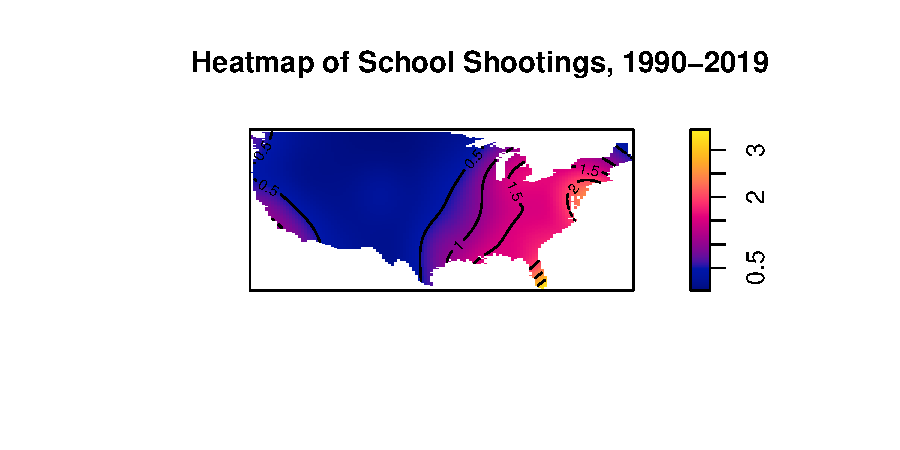
\includegraphics{JStevenRaquel_STATS295_Final_files/figure-latex/density-90-19-1.pdf}

\hypertarget{nearest-neighbor}{%
\subsection{Nearest Neighbor}\label{nearest-neighbor}}

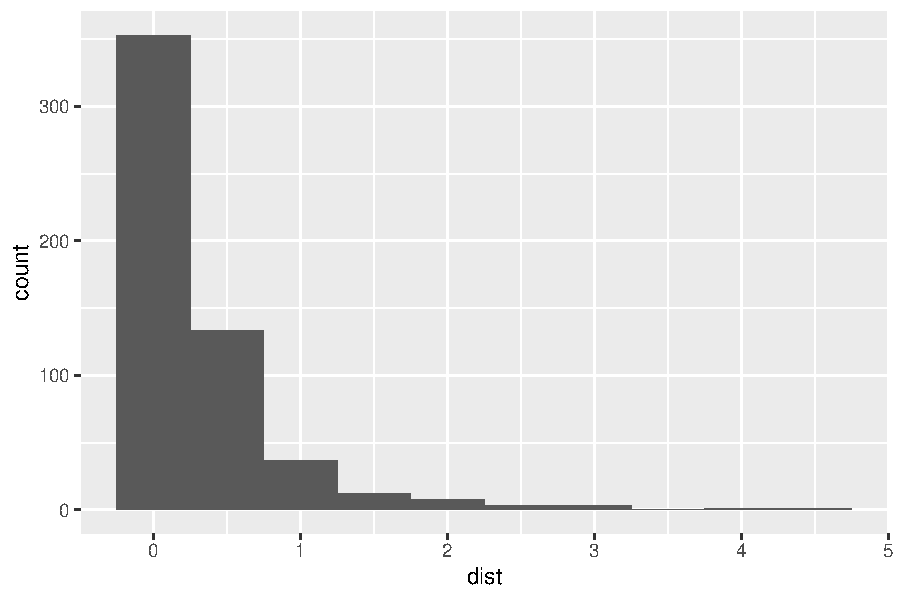
\includegraphics{JStevenRaquel_STATS295_Final_files/figure-latex/nearest-neighbor-1.pdf}

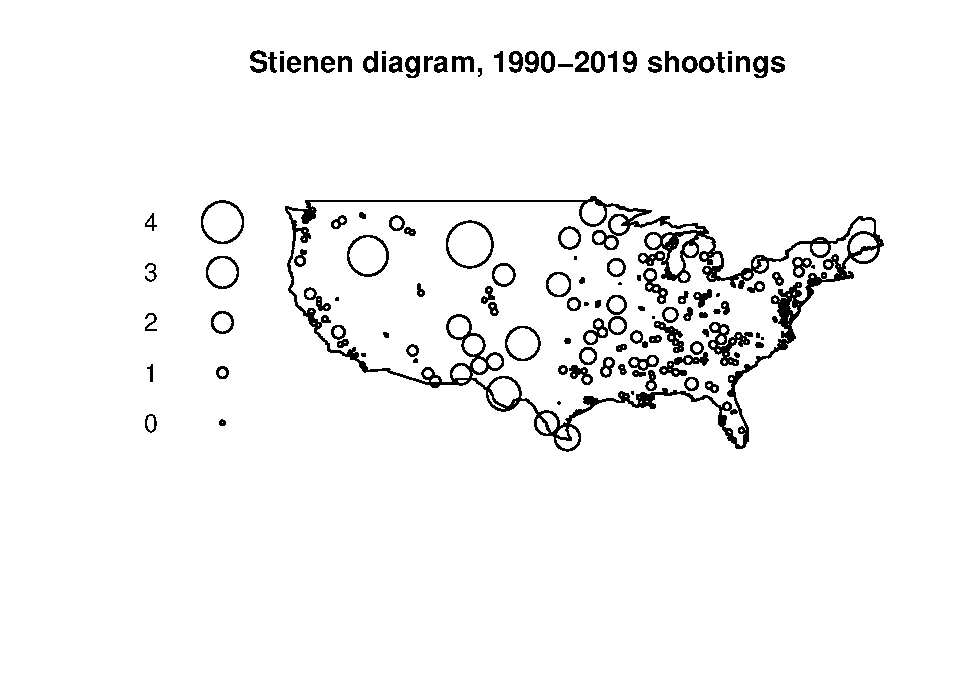
\includegraphics{JStevenRaquel_STATS295_Final_files/figure-latex/Sienen-diagram-1.pdf}

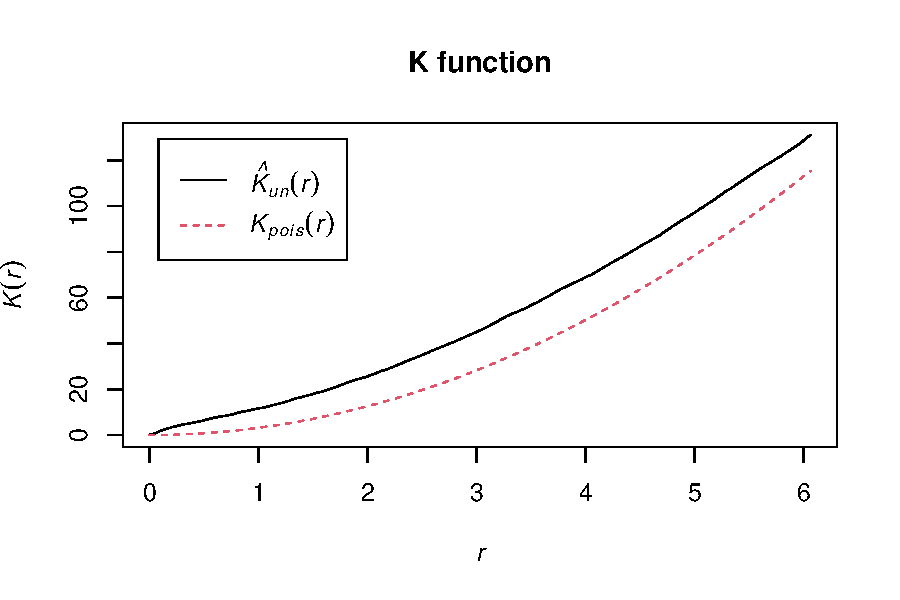
\includegraphics{JStevenRaquel_STATS295_Final_files/figure-latex/K-function-1.pdf}

\begin{verbatim}
## Registered S3 method overwritten by 'imager':
##   method      from
##   plot.imlist
\end{verbatim}

\begin{verbatim}
## Image. Width: 664 pix Height: 664 pix Depth: 1 Colour channels: 3
\end{verbatim}

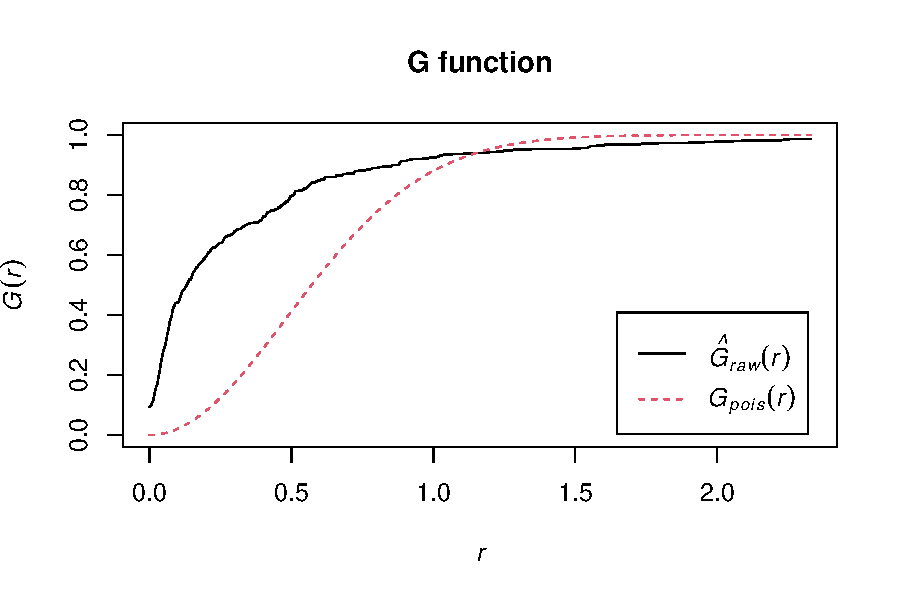
\includegraphics{JStevenRaquel_STATS295_Final_files/figure-latex/G-function-1.pdf}

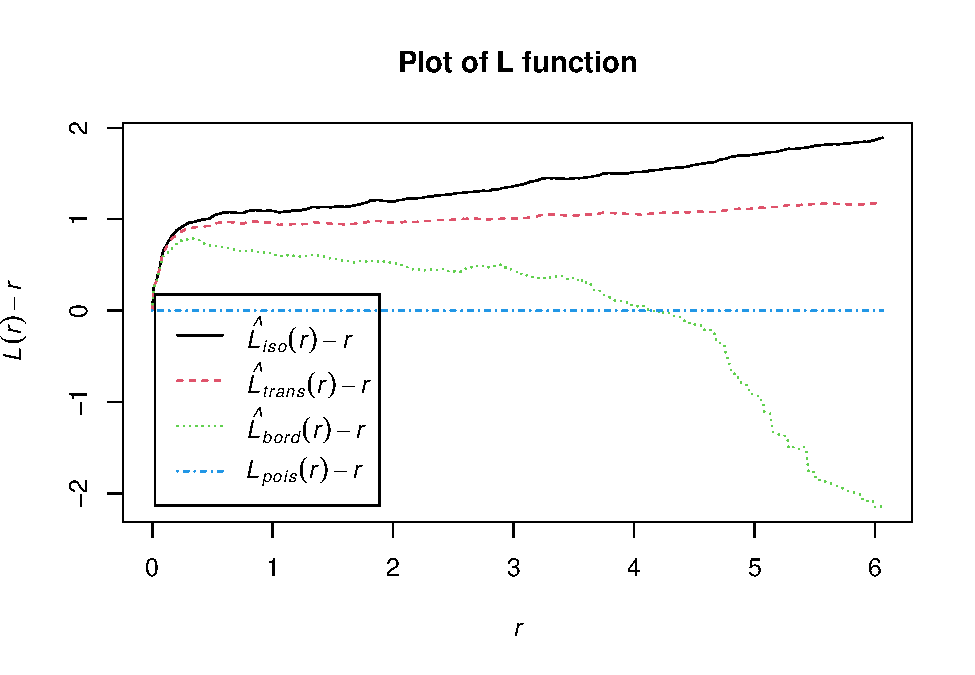
\includegraphics{JStevenRaquel_STATS295_Final_files/figure-latex/KL-functions-1.pdf}

\hypertarget{modeling-the-intensity-function-using-categorical-covariates}{%
\subsection{Modeling the intensity function using categorical covariates}\label{modeling-the-intensity-function-using-categorical-covariates}}

\hypertarget{discussion}{%
\section{Discussion}\label{discussion}}

\newpage

\hypertarget{references}{%
\section{References}\label{references}}

\newpage

\bibliographystyle{agsm}
\bibliography{}


\end{document}
